\subsubsection{Create a course:}

\begin{figure}[H]
	\begin{subfigure}{0.70\linewidth}
		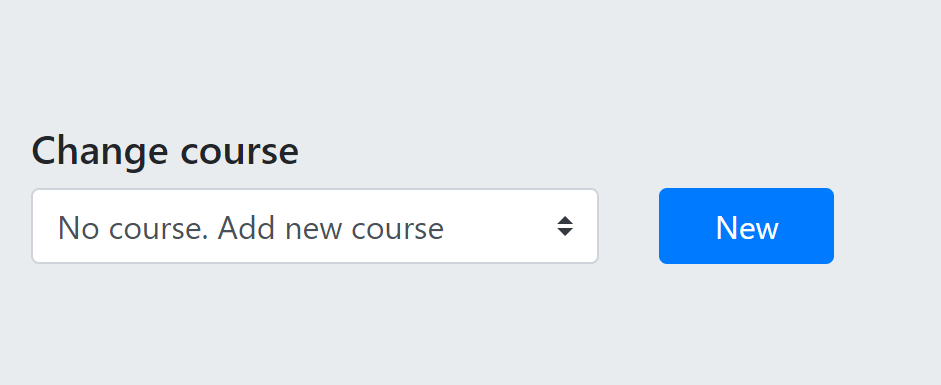
\includegraphics[width=\linewidth]{userManual/adminImages/createCourseDashboard}
		\caption{}
		\label{fig:createCourseDashboard}
	\end{subfigure}
	\begin{subfigure}{0.70\linewidth}
		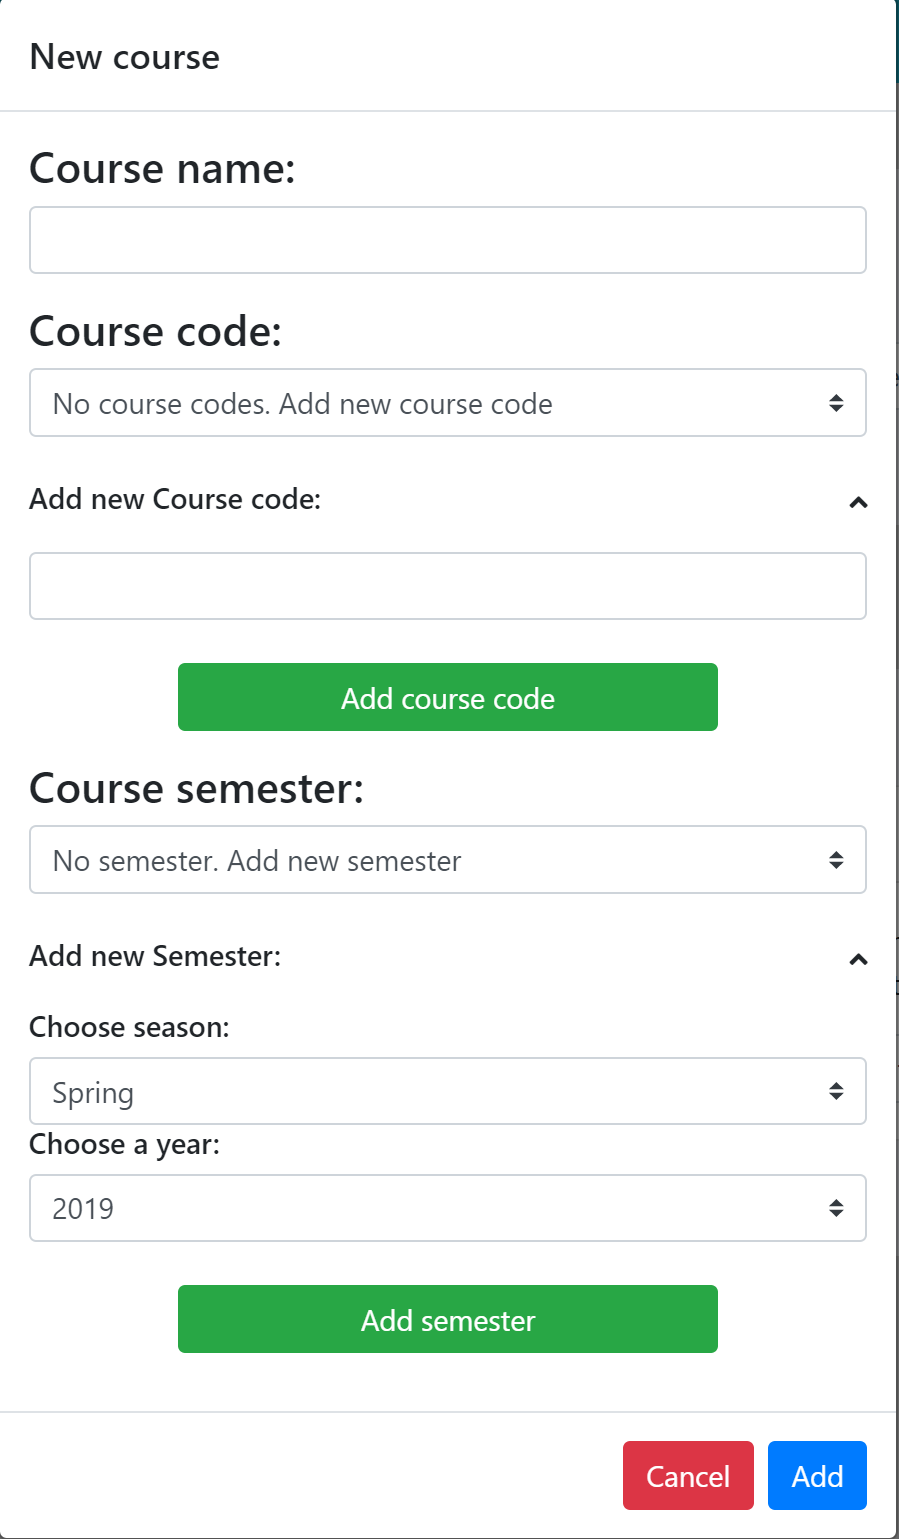
\includegraphics[width=\linewidth]{userManual/adminImages/createNewCourse}
		\caption{}
		\label{fig:createNewCourse}
	\end{subfigure}
\end{figure}

\begin{userManualItemlist}
    \item[Step I.] Navigate to the admin dashboard page.
    \item[Step II]. Click the "New" button (Figure: \ref{fig:createCourseDashboard}).
    \item[-] The following steps reference figure: \ref{fig:createNewCourse}. 
    \item[Step III.] Type the course name.
    \item[Step IV.] Click the "Add new Course Code" field.
    \item[Step V.] Type the course code and click the "Add course code" button.
    \item[Step VI.] If the course semester already exists, select it from the list and click the "Add" button.
    \item[Step VII.] If it does not, create a new semester by clicking on the "Add new Semester" button.
    \item[Step VII.] Select a season in the first select element.
    \item[Step VIII.] Select a year in the second select element.
    \item[Step IX.] Click the "Add semester" button.
    \item[Step X.] Click the "Add" button.    
\end{userManualItemlist}